\chapter{Curved Spacetimes and Gravity}\label{chap:GR}
Our current understanding of gravity is manifested in Einsteins theory of General Relativity. In contrast to the treatment of the other fundamental forces, which are all described by gauge theories and summarized in the Standard Model of Particle Physics, gravity is based on the concept of curved spacetime. This chapter summarizes some of the general concepts and notions of General Relativity, needed for a basic understanding of the subject. For most of the concepts we present here, we are following Sean Carroll's lecture notes \cite{CarrollGR}. At the end of this chapter, we show why gravity can not be quantized in a perturbative manner, in opposition to the other three fundamental forces. For this part we follow \cite{PawlowskiNPgaugeLecture}. 

\section{An Introduction to Spacetime Geometry}
 When talking about the concept of curved spacetimes, one first needs a mathematical framework to quantify curvature and to understand how mathematical concepts such as differentiation and integration are generalized to curved spaces. 
 The central objects in our discussion of curved spaces are \textit{differentiable manifolds}, i\,e. topological spaces, that are  locally diffeomorphic to $\mathbb{R}^n$. Locally in this sense means, that we can find coordinate maps $\phi_i: M \underset{\mathrm{open}}{\supset} U_i \rightarrow \mathbb{R}^n$, such that the image $\phi_i(U_i)$ is open in  $\mathbb{R}^n$, for every point on $M$, whereas globally the manifold may have a very complicated topology. A set of such coordinate maps $\{(U_{\alpha}, \phi_{\alpha})\}$ that covers the entire manifold and where the charts are smoothly sewed together is called an \textit{atlas}. For overlapping charts $U_{\alpha}\cap U_{\beta} \neq \emptyset$, the maps $(\phi_{\alpha} \circ \phi_{\beta}^{-1})$, a.\,k.\,a. coordinate transformations, must be smooth and differentiable. They are directly connected to the coordinates $x^{\mu}$ we'll work with later on. \\
Further, we need to introduce additional structures, such as vectors and tensors on manifolds, since they are the objects we are interested in when it comes to the discussion of physical models. To be able to talk about vectors, one needs to associate  a \textit{tangent space} $T_p$ to every point $p$ of the manifold. The tangent space is the set of all vectors at  $p$ and  has the structure of a vector space with the same dimension as $M$. The disjoint union of all tangent spaces on $M$ is called the \textit{tangent bundle}. To specify the concept of the tangent space we claim, that it can be identified with the space of directional derivative operators along curves $\gamma: \mathbb{R} \rightarrow M$  through $p$. In this case, we find a basis of $T_p$ as the set $\{\hat{\partial}_{\mu}\}$ of directional derivatives at $p$. It can be shown, that the directional derivatives can be decomposed into a sum of real numbers times partial derivatives, i.\,e. $\frac{d}{d \lambda} = \frac{d x^{\mu}}{d \lambda}\partial_{\mu}$, where $\lambda$ is the parameter of the curve $\gamma$. This allows us to represent a vector $V=V^{\mu}\partial_{\mu}$ independently of the chosen coordinates. The basis vectors in some different coordinate system $x^{\mu^{\prime}}$ are then simply related to the initial basis via $\partial_{\mu^{\prime}}=\frac{\partial x^{\mu}}{\partial x^{\mu^{\prime}}} \partial_{\mu}$ which yields the transformation law for vector components under general coordinate transformations,
\begin{align}
	V^{\mu^{\prime}}=\frac{\partial x^{\mu^{\prime}}}{\partial x^{\mu}} V^{\mu}. \label{eqn:contravariant_trafo}
\end{align}
Components obeying this transformation law are called \textit{contravariant}. At this point it follows quite naturally to define the \textit{cotangent space} $T_p^*$ as the set of linear maps $\omega: T_p \rightarrow \mathbb{R}$. Elements of the cotangent space are called one-forms or dual vectors and similarly to the discussion of the tangent space, we find a suitable basis for $T_p^*$ as the gradients $\{\dd\hat{x}^{\mu}\}$, allowing us to represent arbitrary one-forms as $\omega = \omega_{\mu} \dd x^{\mu}$. As before, we are interested in the transformation behavior of our basis one-forms, i.\,e. $\mathrm{d} x^{\mu^{\prime}}=\frac{\partial x^{\mu^{\prime}}}{\partial x^{\mu}} \mathrm{d} x^{\mu}$, and the dual vector components
\begin{align}
	\omega_{\mu^{\prime}}=\frac{\partial x_{\mu}}{\partial x^{\mu^{\prime}}} \omega_{\mu}.\label{eqn:covariant_trafo}
\end{align}
This transformation behavior differs from the one found for vectors. We call components transforming as in equation (\ref{eqn:covariant_trafo}) \textit{covariant}.
Now we are able to generalize these concepts by introducing tensors $T$ of type $(k,l)$ as
\begin{align}
T=T_{\phantom{\mu_{1} \cdots \mu_{k}}\nu_{1} \cdots \nu_{l}}^{\mu_{1} \cdots \mu_{k}} \ \partial_{\mu_{1}} \otimes \cdots \otimes \partial_{\mu_{k}} \otimes \mathrm{d} x^{\nu_{1}} \otimes \cdots \otimes \mathrm{d} x^{\nu_{l}}.
\end{align}
Here $\otimes$ denotes the usual tensor product.
The general transformation law for tensors follows naturally as expected from equations (\ref{eqn:contravariant_trafo}) and (\ref{eqn:covariant_trafo}),
\begin{align}
	T_{\phantom{\mu_{1}^{\prime} \cdots \mu_{k}^{\prime}}\nu_{1}^{\prime} \cdots \nu_{l}^{\prime}}^{\mu_{1}^{\prime} \cdots \mu_{k}^{\prime}}=\frac{\partial x^{\mu_{1}^{\prime}}}{\partial x^{\mu_{1}}} \cdots \frac{\partial x^{\mu_{k}^{\prime}}}{\partial x^{\mu_{k}}} \frac{\partial x^{\nu_{1}}}{\partial x^{\nu_{1}^{\prime}}} \cdots \frac{\partial x^{\nu_{l}}}{\partial x^{\nu_{l}^{\prime}}} T^{\mu_{1} \cdots \mu_{k}}_{\phantom{\mu_{1} \cdots \mu_{k}}\nu_{1} \cdots \nu_{l}}.
\end{align}
Having understood the basic structures and their respective behavior under coordinate transformations, we are now able to present some of the most important tensors in General Relativity. \\
Maybe the most important object to quantify curved space is the \textit{metric tensor} $g_{\mu\nu}$\footnote{It is convenient to write the components $T_{\phantom{\mu_{1} \cdots \mu_{k}}\nu_{1} \cdots \nu_{l}}^{\mu_{1} \cdots \mu_{k}}$ when speaking about tensors $T$.} and its inverse  $g^{\mu\nu}$, related via $g^{\mu\nu}g_{\nu\sigma} = \delta^{\mu}_{\phantom{\mu}\sigma}$. The metric and its inverse can be used to raise and lower indices, e.\,g. $x^{\mu} = g^{\mu\nu}x_{\nu}$. Additionally we can compute path lengths and proper time via the definition of the line element 
\begin{align}
	\dd s^{2}=g_{\mu \nu} \mathrm{d} x^{\mu} \mathrm{d} x^{\nu}.
\end{align}
\begin{minipage}{\textwidth}
	For arbitrary vector fields $V$ and $W$ the scalar product induced by the metric tensor \\ reads
\vspace{-0.4cm}
\begin{align}
	g(V,W) = g_{\mu\nu}V^{\mu}W^{\nu} = V^{\mu}W_{\mu}= g^{\mu\nu}V_{\mu}W_{\nu} = V_{\mu}W^{\mu}.
\end{align}
\end{minipage}\vfill\newpage
We will see, that the metric tensor already contains all the information on the geometrical structure of the respective manifold, whose curvature we want to quantify. Nevertheless, we first have to think about differentiation of general tensors again. \\
In flat space, the partial derivative is a map from $(k, l)$ to $(k, l+1)$ tensor fields satisfying linearity and the Leibniz product rule. We want to generalize this concept to curved space by introducing the \textit{covariant derivative} $\nabla$\footnote{In the context of quantum field theory, the gauge covariant derivative is often written as $D$. Nevertheless, throughout this thesis we will use $\nabla$ to indicate any kind of covariant derivative.}. In contrast to the usual partial derivative, the covariant derivative is independent of the chosen set of coordinates. Consider for example the covariant derivative of a vector field $V$, which can be written as a partial derivative plus some correction term due to its property to obey the Leibniz rule:
\begin{align}
\nabla_{\mu} V^{\nu}=\partial_{\mu} V^{\nu}+\Gamma_{\phantom{\nu}\mu \lambda}^{\nu} V^{\lambda}.
\label{eqn:cov_deriv}
\end{align}
Here, the correction term is specified by the so-called \textit{Christoffel symbols}, a.\,k.\,a. \textit{connection coefficients}. They are determined by derivatives of the metric tensor:  
\begin{align}
\Gamma_{\phantom{\alpha}\mu \nu}^{\alpha}=\frac{1}{2} g^{\mu \lambda}\left(\partial_{\mu} g_{\nu \lambda}+\partial_{\nu} g_{\mu \lambda}-\partial_{\lambda} g_{\mu \nu}\right)\footnotemark.	
\end{align}
\footnotetext{This holds only true, if the connection is \textit{torsion free}, i.\,e. $
T_{\phantom{\lambda}\mu \nu}^{\lambda}=\Gamma_{\phantom{\lambda}\mu \nu}^{\lambda}-\Gamma_{\phantom{\lambda}\nu \mu}^{\lambda}=2 \Gamma_{\phantom{\lambda}[\mu \nu ]}^{\lambda} = 0$, and fullfils \textit{metric compatibility}, i.\,e.$
\nabla_{\rho} g_{\mu \nu}=0$. For the most important connection in the context of General Relativity, the \textit{Levi-Civita connection}, these properties are fullfilled. The fundamental theorem of Riemannian geometry states, that for every Riemannian manifold there exists a unique Levi-Civita connection. It is determined by the Koszul formula.}
It can be shown, that the connection coefficients themselves do \textit{not} transform like tensor components, but are constructed in a way such that the combination (\ref{eqn:cov_deriv}) does. Note, that the covariant derivative reduces to the partial when applied to scalars. With this definition of the connection, we are now finally able to introduce the remaining tensor structures needed for the understanding of the calculations presented later on in this work. \\
The central object in our discussion of curvature is the \textit{Riemann tensor} $R_{\phantom{\alpha}\beta \gamma \delta}^{\alpha}$. It is a $(1, 3)$-tensor given by
\begin{align} 
	R_{\phantom{\alpha}\beta \gamma \delta}^{\alpha}=\partial_{\gamma} \Gamma_{\phantom{\alpha}\beta \delta}^{\alpha}-\partial_{\delta} \Gamma_{\phantom{\alpha}\beta \gamma}^{\alpha}+\Gamma_{\phantom{\alpha}\beta \delta}^{\epsilon} \Gamma_{\phantom{\alpha}\epsilon \gamma}^{\alpha}-\Gamma_{\phantom{\alpha}\beta \gamma}^{\epsilon} \Gamma_{\phantom{\alpha}\epsilon \delta}^{\alpha}.
\end{align}
It contains all the information about the curvature of the respective manifold. Another useful definition of the Riemann tensor is related to the commutator of two covariant derivatives, acting on a vector field:
\begin{align}
	\left[\nabla_{\mu}, \nabla_{\nu}\right] A^{\sigma}=R_{\phantom{\alpha}\rho \mu \nu}^{\sigma} A^{\rho}. \label{eqn:Riemann}
\end{align}
We are also interested in contractions of the Riemann tensor, especially the \textit{Ricci tensor} 
\begin{align}
	R_{\mu\nu} = R^{\alpha}_{\phantom{\alpha}\mu\alpha\nu} = g_{\alpha\beta} R^{\beta}_{\phantom{\alpha}\mu\alpha\nu}
\end{align}
and the \textit{Ricci scalar} 
\begin{align}
\mathcal{R} = g_{\mu\nu}R^{\mu\nu} = R^{\mu}_{\phantom{\mu}\mu}.
\end{align}
At this point, we also want to introduce the \textit{Einstein tensor}, defined as
\begin{align}
	 G_{\mu\nu} = R_{\mu\nu} - \frac{1}{2}g_{\mu\nu}\mathcal{R}.
\end{align}
Having introduced the setup for the calculations performed in this work, we are now ready to introduce the \textit{Einstein-Hilbert action}, providing the starting point for an investigation of quantum gravity within the Functional Renormalization Group approach. 
\section{From Geometry to Einsteins Equations}
The Einstein-Hilbert action, given by
\begin{align}
	\mathcal{S}_{\text{EH}} = \frac{1}{16\pi G} \int_x \sqrt{g} \ (\Ricci - 2\Lambda), 
\end{align}
where $G$ is Newtons coupling and $\Lambda$ is the cosmological constant, describes a minimally coupled theory of gravity, leading to a $\sfrac{1}{r}$ gravitational potential in the non-relativistic limit. Note, that compared to the usual spacetime measure a factor of $\sqrt{g} := \sqrt{-\operatorname{det}g_{\mu\nu}}$ is included to preserve diffeomorphism invariance.\footnote{Diffeomorphism invariance, i.\,e. the freedom of choosing an appropriate coordinate system, is the central symmetry in the context of General Relativity, based  on the assumption, that coordinates do not exist a priori in nature, but are rather a mathematical tool used to describe it, that should not change the fundamental laws of physics.\nopagebreak} \\ 
Varying the Einstein-Hilbert action w.\,r.\,t. the inverse metric $g^{\mu\nu}$ yields Einsteins equations in absence of matter:
\begin{align}
	G_{\mu\nu} + \Lambda g_{\mu\nu} = 0.
\end{align}
The non-vacuum Einstein equations are obtained the same way, after the inclusion of matter in this setting  by adding a matter part to the Einstein-Hilbert action:
\begin{equation}
	\mathcal{S} = \frac{1}{8\pi G}\mathcal{S}_{\mathrm{EH}} + \mathcal{S}_{\text{matter}}.
\end{equation}
With the definition of the Energy-Momentum tensor $T_{\mu\nu}$, given by
\begin{align}
	T_{\mu\nu} = \frac{-2}{\sqrt{g}} \frac{\delta\mathcal{S}_{\text{matter}}}{\delta g^{\mu\nu}},
\end{align}
we arrive at 
\begin{align}
\frac{1}{8\pi G}\left[G_{\mu\nu} + \Lambda g_{\mu\nu}\right] = T_{\mu\nu}.	
\end{align}
In this form, Einsteins equations perfectly embody the direct correlation between curvature (l.\,h.\,s.) and the dynamics of the matter content of the theory (r.\,h.\,s.). \\
At the end of this chapter we want to emphasize the problem of perturbative non-renormali- zability in the context of finding a quantum field theoretical description of gravity. 
\section{Perturbative Non-Renormalizability of Gravity}
Naively, one could try to quantize gravity via the path integral formalism with a generating functional, given by $\int_{g_{\mu\nu}} \operatorname{e}^{-\mathcal{S}_{\mathrm{EH}}}$, as usual. The main problem in this approach is the lack of positivity of $\mathcal{S}_{\mathrm{EH}}$ causing problems with unitarity of the theory. In quantum gravity one usually introduces a linear split of the \textit{full} metric $g_{\mu\nu}$, to perform expansions about a given background $\bar{g}_{\mu\nu}$, comparable to classical perturbation theory, which is based on coupling or amplitude expansions around the free Gaussian theory. The linear split reads
\begin{align}
	g_{\mu\nu} = \bar{g}_{\mu\nu} + \sqrt{G}h_{\mu\nu},
	\label{eqn:metric_split}
\end{align}
with the metric fluctuation $h_{\mu\nu}$ defined as $h_{\mu\nu}= 1/\sqrt{G}\left(g_{\mu\nu}-\bar{g}_{\mu\nu}\right)$. This allows us to write the path integral in terms of the fluctuation field as
\begin{equation}
Z\left[J^{\mu \nu} ; \overline{g}_{\mu \nu}\right] \propto \int_{h_{\mu \nu}} \operatorname{e}^{-S_{\mathrm{EH}}\left[\bar{g}_{\mu \nu}+\sqrt{G} h_{\mu \nu}\right]+\int_x \sqrt{\bar{g}} \  J^{\mu \nu} h_{\mu \nu}}.
\end{equation}
Note, that the source term depends on the determinant of the background metric, otherwise the usual $J^{\mu\nu}$ derivatives would not generate the $n$-point functions of the fluctuation field $h_{\mu\nu}$. We will come back to this problem, which is often referred to as \textit{background independence}, at the end of this thesis in chapter \ref{chap:BGindependence}. \\
After a suitable tensor decomposition of the fluctuation field and a gauge fixing procedure \`a la Faddeev-Popov\footnote{The functional quantization of gauge theories requires a gauge fixing procedure due to redundancies in the path integral measure. The idea of Faddeev and Popov is to represent the gauge fixing condition, which is implemented in the functional integral, as an additional functional integral over a set of Grassmann fields $c$ and $\bar{c}$, known as \textit{Faddeev-Popov ghosts}. Even though they are anticommuting Grassmann fields, they transform as scalars under Lorentz transformations. They also violate spin statistics. Nevertheless, they can be treated as additional particles in the computation of Feynman diagrams. For a detailed discussion, see e.\,g. ch. 16 in \cite{PeskinSchroeder1995} or  sec. 5.2 in \cite{PawlowskiNPgaugeLecture}.},  we are left with the gauge fixed Einstein-Hilbert action
\begin{align}
	\mathcal{S}_{\text{grav}}[\bar{g},\Phi] = \mathcal{S}_{\text{EH}}[g] + \mathcal{S}_{\text{gf}}[\bar{g}, h] + \mathcal{S}_{\text{gh}}[\bar{g},\Phi] .
\end{align}
 Here the pure gravity multi-field $\Phi=(h_{\mu\nu}, c_{\mu}, \bar{c}_{\mu})$ was introduced. Altogether, this yields the gauge-fixed path integral representation of quantum gravity:
 \begin{equation}
Z[J ; \bar{g}]=\int_{\Phi} \operatorname{e}^{-\mathcal{S}_{\text{grav}}\left[\bar{g}_{\mu\nu}, \Phi\right]+\int_x \sqrt{\bar{g}} \ J \cdot \Phi}.
\end{equation}
An analysis of the canonical momentum dimensions of the essential couplings of this theory, $G$ and $\Lambda$, results in:
\begin{equation}
\left[G\right] = \left[\dd^dx \sqrt{g}\ \mathcal{R}\right] = 2-d,  \qquad\qquad\qquad \left[\Lambda\right] = 2.
\end{equation}
This implies, that the Newton coupling has a negative mass dimension in $d=4$ spacetime dimensions. To investigate the consequences of this, one can consider the grade of divergence $\Lambda^{\delta(\gamma)}$ for a general graph $\gamma$ with $E$ external lines, $I$ internal propagators and $L$ loops. Here, $\Lambda$ is an UV cutoff for the momentum integrals and $\delta(\gamma)$ is the index of the graph,
\begin{equation}
	\delta(\gamma) = dL- 2\left(I-\sum_{n=3}^{\infty}\nu_n\right),
\end{equation}
where the $\nu_n$ represent $n$-graviton vertices. After expressing the number of loops in terms of the internal lines and the $n$-graviton vertices and restricting ourselves to graphs satisfying $E + 2I = \sum_{n=3}^{\infty}\nu_n$, we find
\begin{equation}
	\delta(\gamma)=d-\frac{d-2}{2} E+\sum\limits_{n=3}^{\infty} v_{n} \delta\left(v_{n}\right),
\end{equation}
where $\delta\left(v_{n}\right)=\frac{1}{2}(n-2)(d-2)$.
After fixing the number of external lines, e.\,g. to $E=2$, representing the case of vacuum polarization as depicted in figure (\ref{fig:vacuum_pol}), one is now able to investigate the grade of divergence for diagrams of different loop orders. t'Hooft and Veltman proved that the theory is renormalizable up to 1-loop order \cite{tHooftVeltmann1974}, but already at 2-loop order, Goroff and Sagnotti showed, that non-vanishing counterterms are generated \cite{GoroffSanotti1985}. In general, this is interpreted as the failure of perturbative quantization of gravity due to the negative mass dimension of the Newton coupling. This leads us to our discussion of Asymptotic Safety as a non-perturbative approach based on the FRG we presented in the last chapter.  

\begin{figure}[t]
\centering
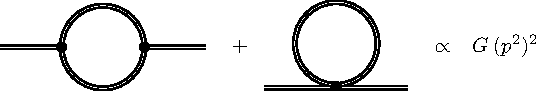
\includegraphics[width=0.8\textwidth]{figs/TikZ/vacuum_pol}
\caption[Vacuum polarization diagrams up to $1$-loop order.]{Vacuum polarization diagrams up to $1$-loop order. The double lines represent the graviton propagator.}	
\label{fig:vacuum_pol}
\hrulefill
\end{figure}